\section{Results}
\label{results}

The algorithms presented here have been implemented using the  Autodesk\textsuperscript{\textregistered} Inventor's Application Programming Interface (API) in Visual Basic.Net.  Table ~\ref{tbl_fbcmalpha} shows the results of some sample test cases run on an Intel i3 64-bit 2 GHz Windows 7 machine:



\newcommand \myColWidthFactorb {0.31}
\begin{center}
\resizebox{0.6\linewidth}{!}{
%\begin{tabular}[!htb]{@{}p{0.22\linewidth} p{0.22\linewidth}  p{0.22\linewidth}  p{0.22\linewidth} @{}} \toprule
\begin{tabular}[!htb]{@{}p{\myColWidthFactorb\linewidth} p{\myColWidthFactorb\linewidth}   p{\myColWidthFactorb\linewidth} @{}} \toprule
{\bf Part} & {\bf Cellular}  & {\bf Result} \\ \midrule  

\adjustbox{valign=t}{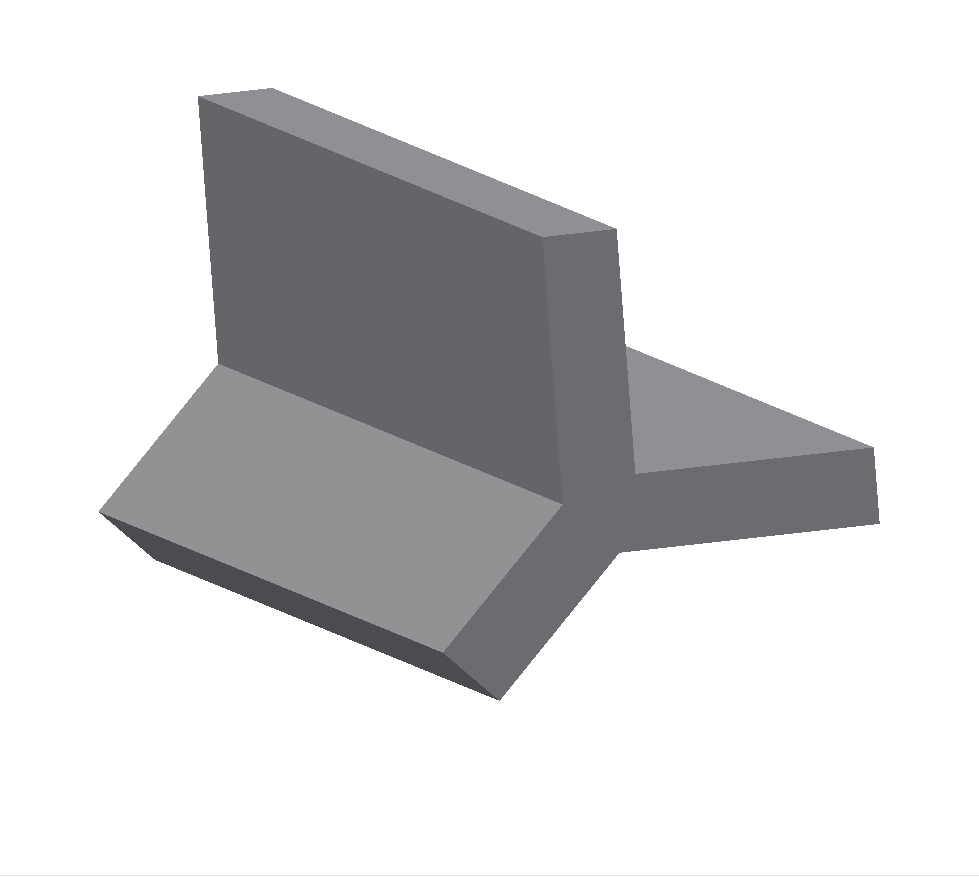
\includegraphics[width=\linewidth]{../Common/images/nonCellular_Y}}  &  
\adjustbox{valign=t}{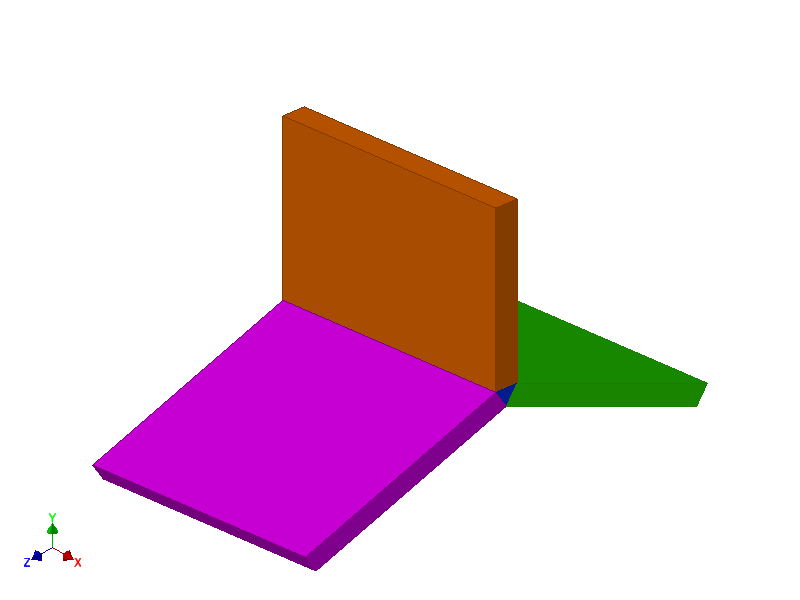
\includegraphics[width=\linewidth]{../Common/images/Cellular_Y}}  &
\adjustbox{valign=t}{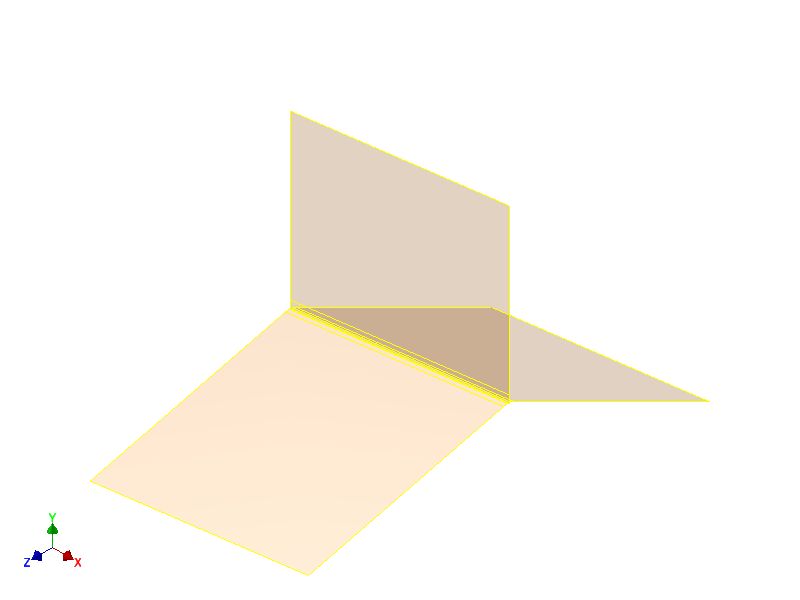
\includegraphics[width=\linewidth]{../Common/images/Cellular_Y_midsurf}} 
\\ \midrule

\adjustbox{valign=t}{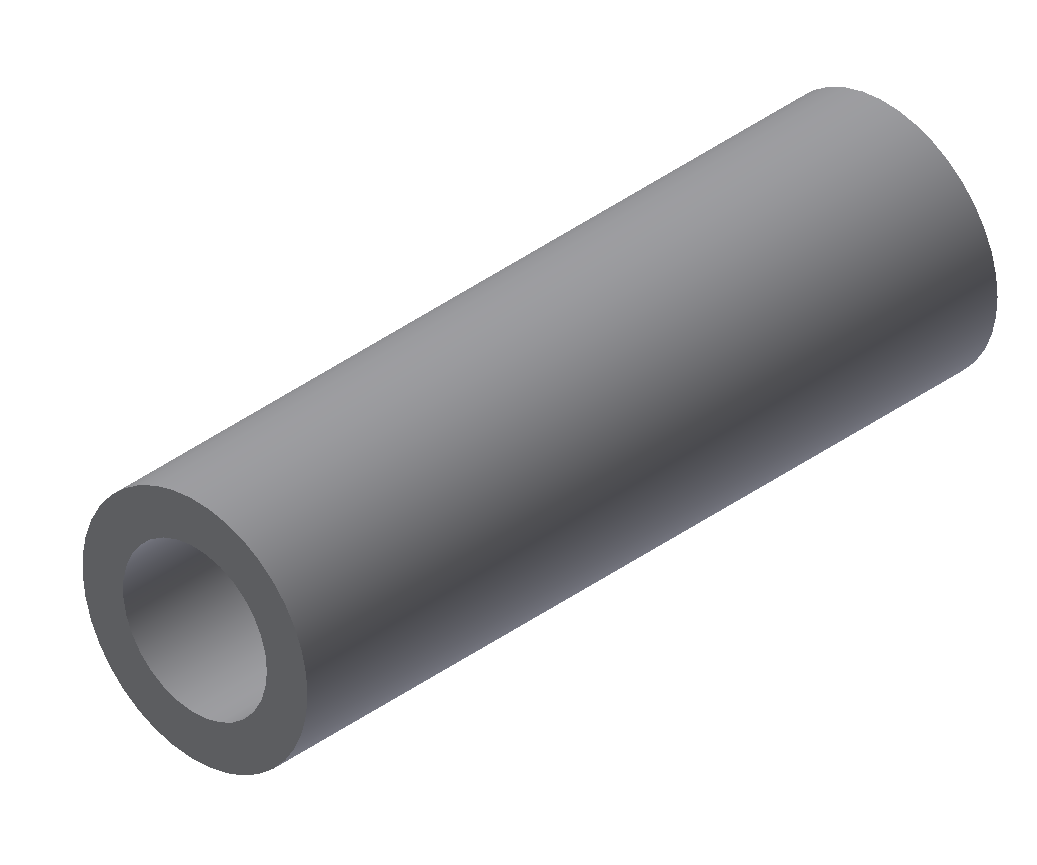
\includegraphics[width=\linewidth]{../Common/images/nonCellular_O}}  &  
\adjustbox{valign=t}{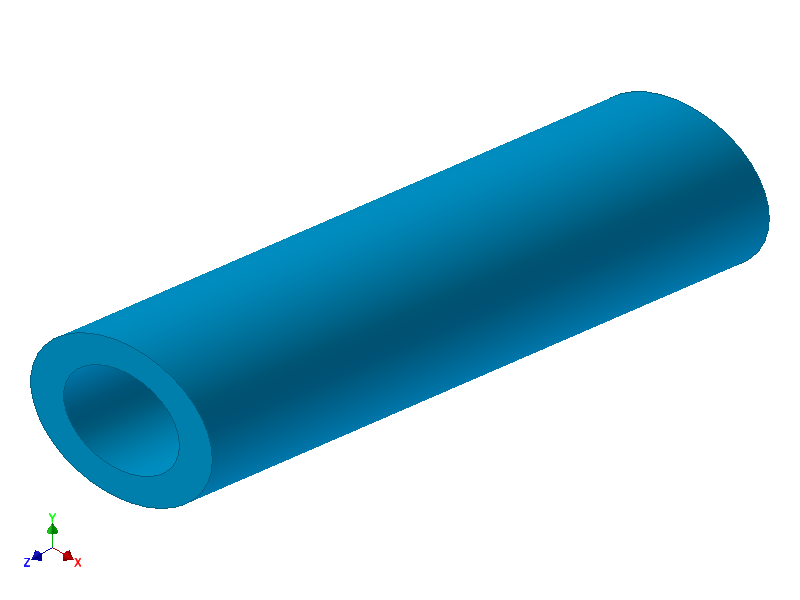
\includegraphics[width=\linewidth]{../Common/images/Cellular_O}}  &
\adjustbox{valign=t}{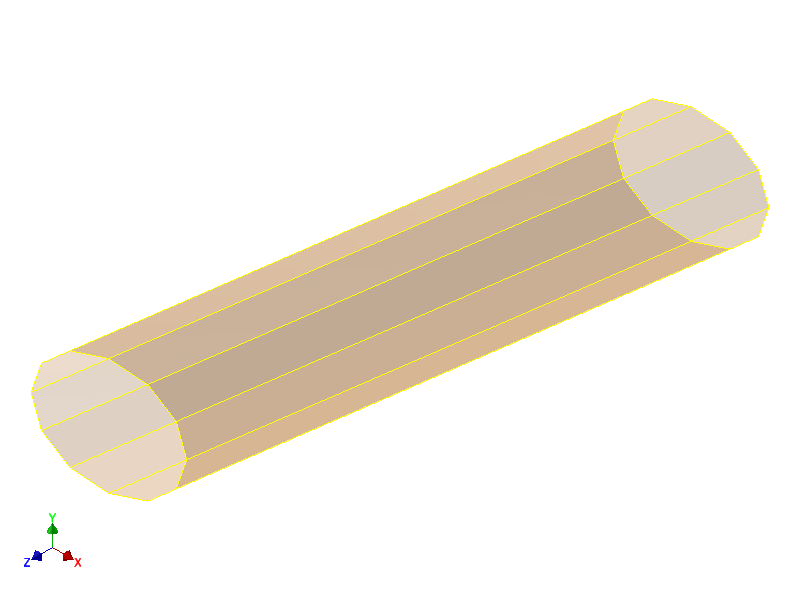
\includegraphics[width=\linewidth]{../Common/images/Cellular_O_midsurf}} 
\\ \midrule

\adjustbox{valign=t}{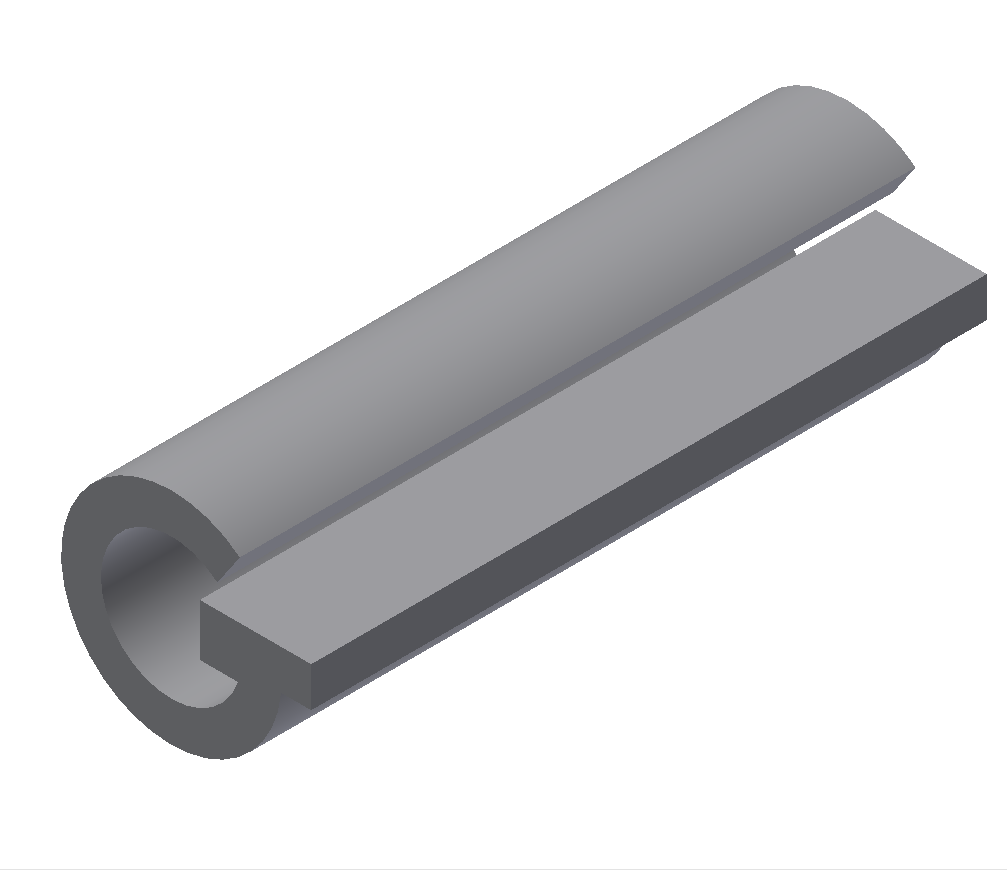
\includegraphics[width=\linewidth]{../Common/images/nonCellular_G}}  &  
\adjustbox{valign=t}{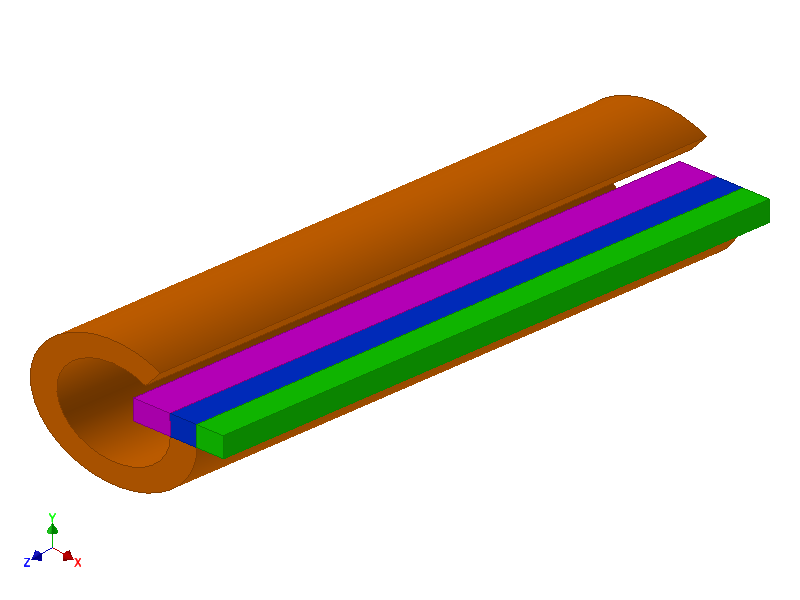
\includegraphics[width=\linewidth]{../Common/images/Cellular_G}}  &
\adjustbox{valign=t}{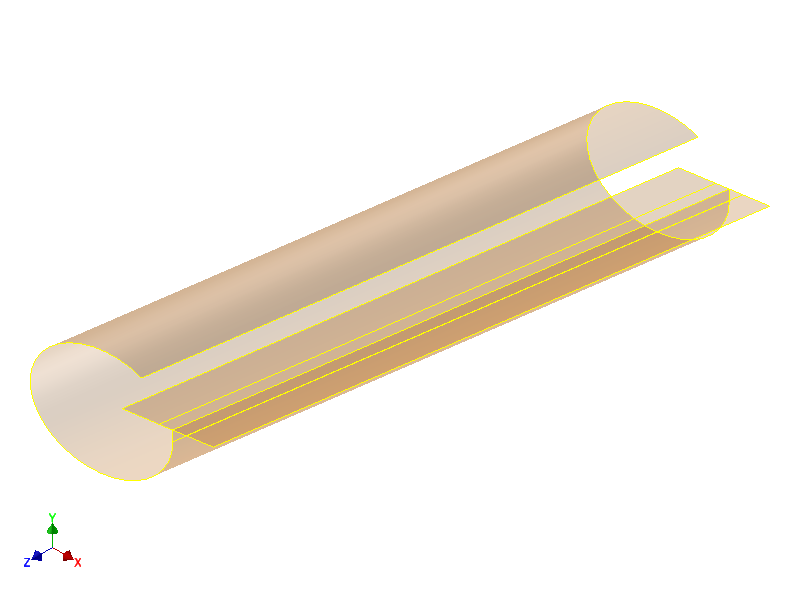
\includegraphics[width=\linewidth]{../Common/images/Cellular_G_midsurf}} 
\\ \midrule

\adjustbox{valign=c}{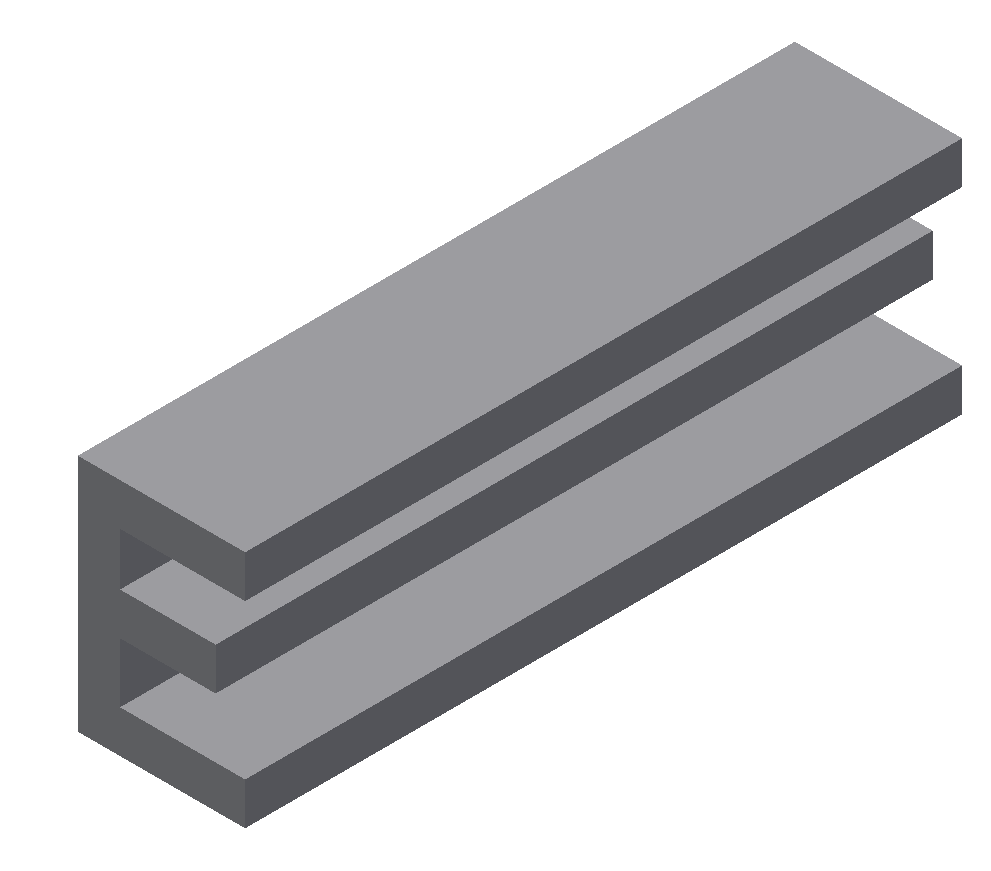
\includegraphics[width=0.8\linewidth]{../Common/images/nonCellular_E}}  &  
\adjustbox{valign=c}{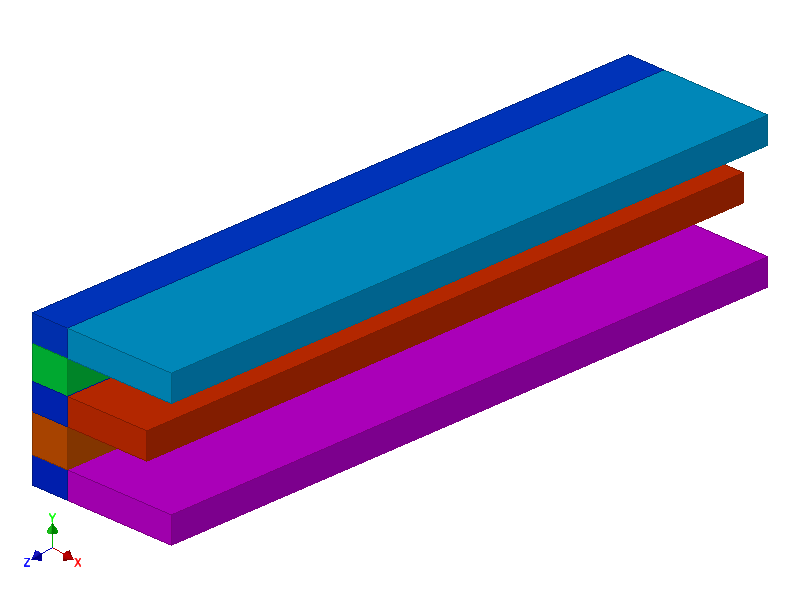
\includegraphics[width=\linewidth]{../Common/images/Cellular_E}}  &
\adjustbox{valign=c}{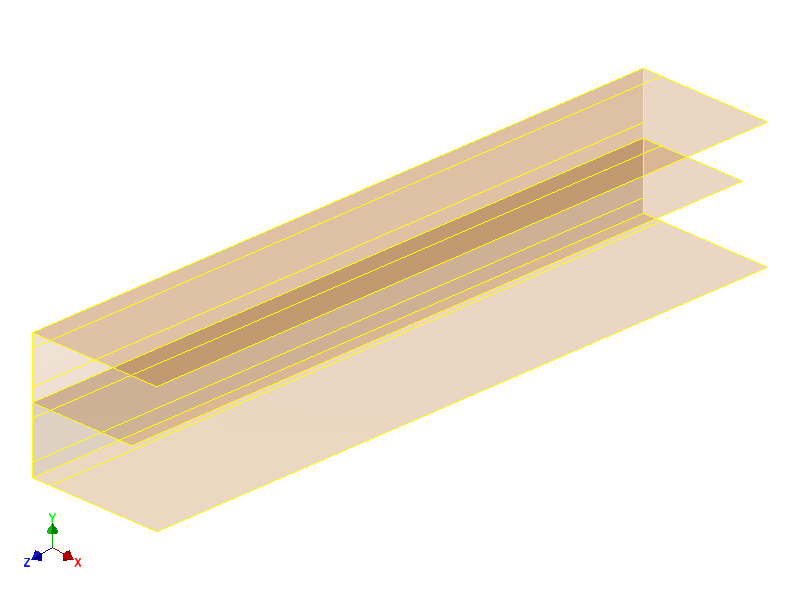
\includegraphics[width=\linewidth]{../Common/images/Cellular_E_midsurf}} 
\\ \midrule


\adjustbox{valign=t}{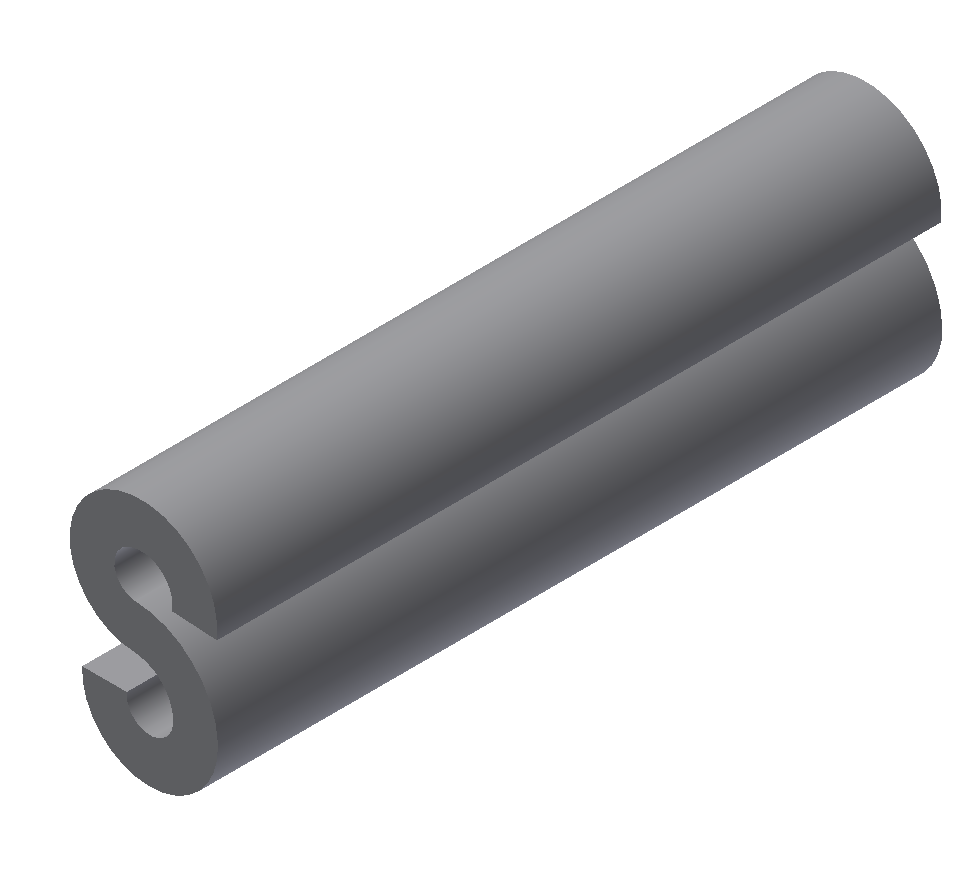
\includegraphics[width=\linewidth]{../Common/images/nonCellular_S}}  &  
\adjustbox{valign=t}{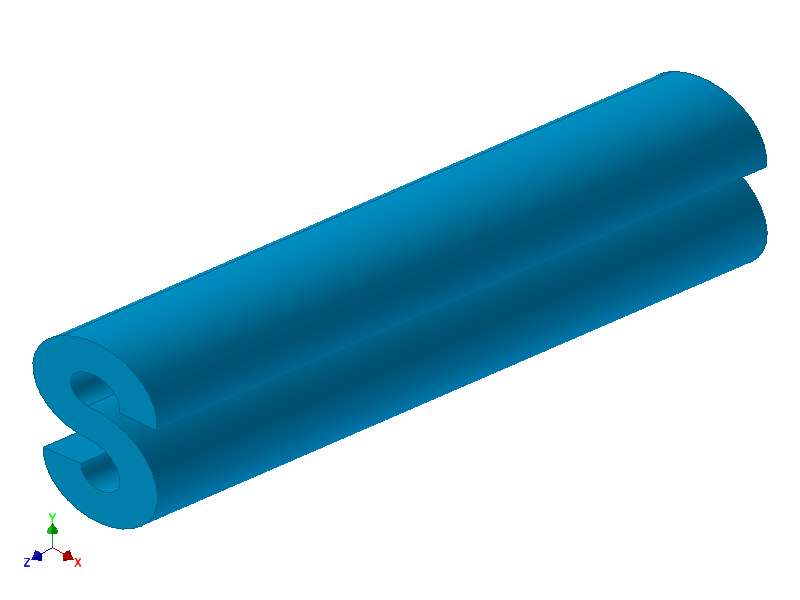
\includegraphics[width=\linewidth]{../Common/images/Cellular_S}}  &
\adjustbox{valign=t}{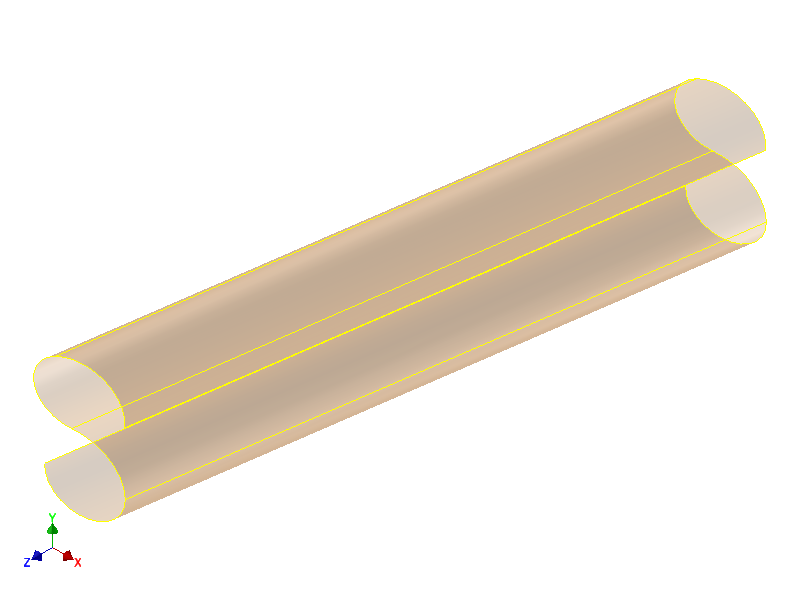
\includegraphics[width=\linewidth]{../Common/images/Cellular_S_midsurf}} 
\\ \midrule


\adjustbox{valign=t}{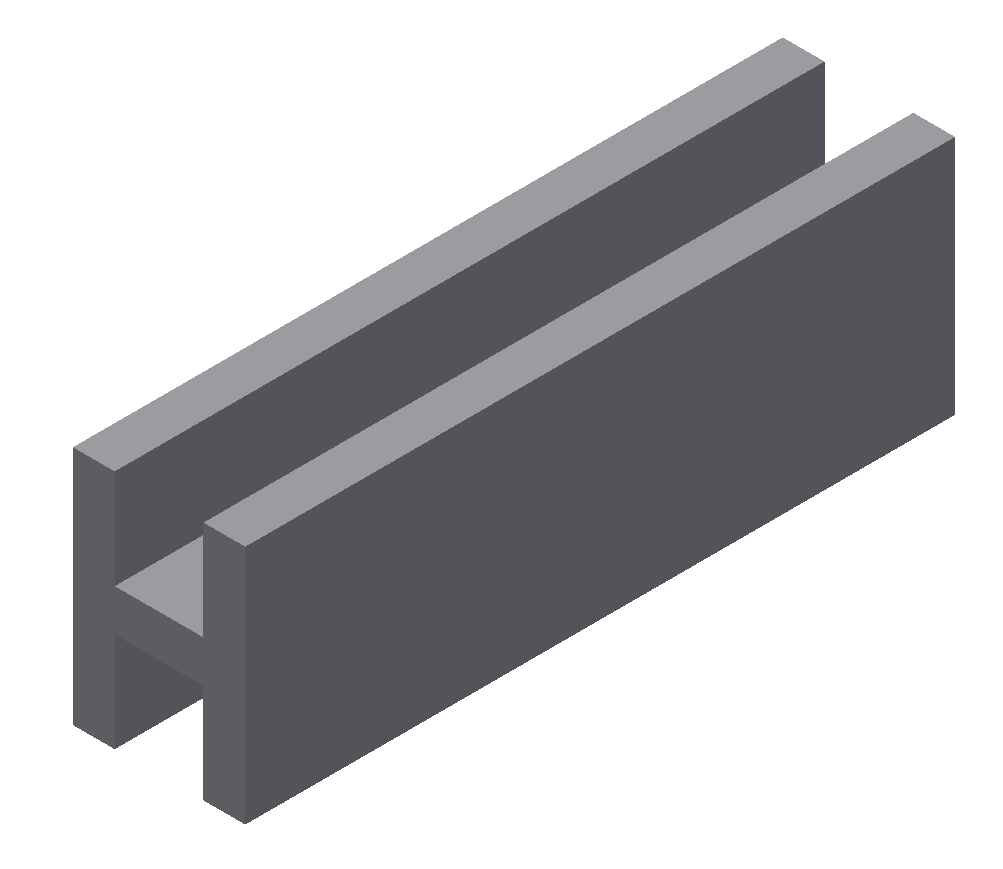
\includegraphics[width=\linewidth]{../Common/images/nonCellular_H}}  &  
\adjustbox{valign=t}{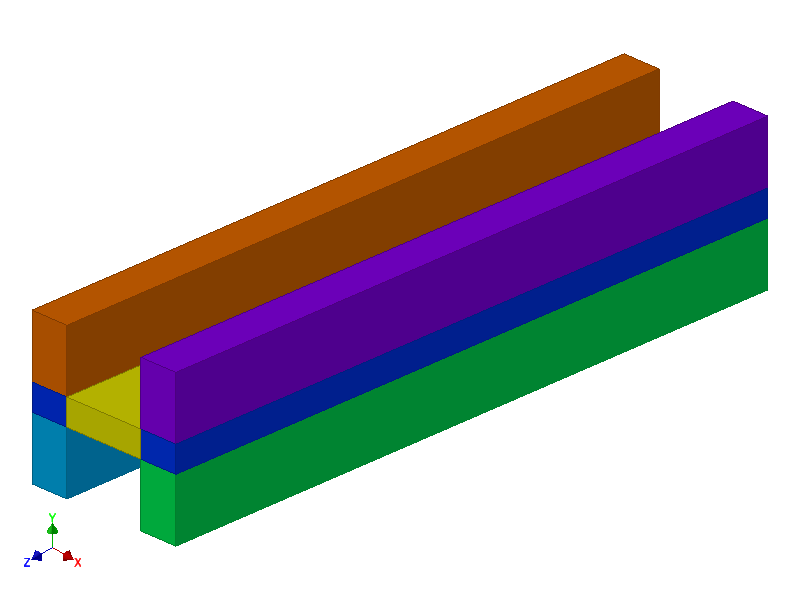
\includegraphics[width=\linewidth]{../Common/images/Cellular_H}}  &
\adjustbox{valign=t}{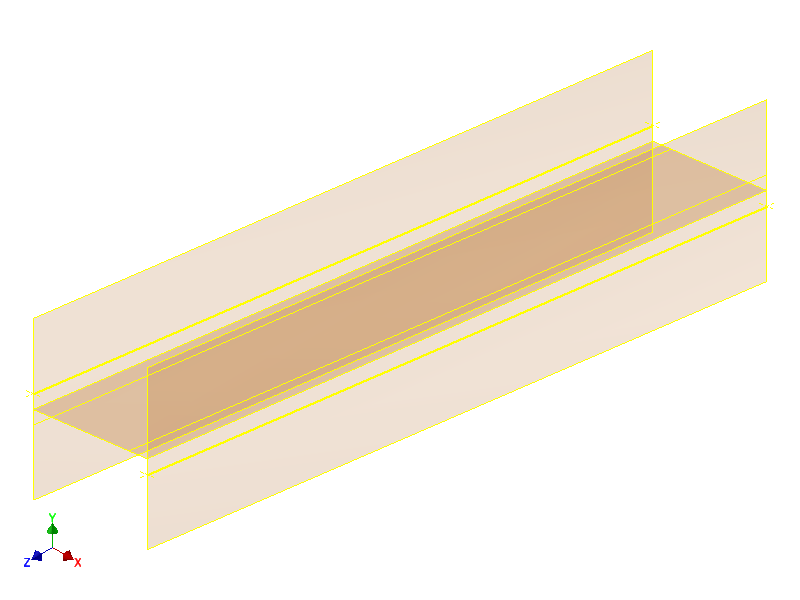
\includegraphics[width=\linewidth]{../Common/images/Cellular_H_midsurf}} 
\\ % \midrule

%\adjustbox{valign=t}{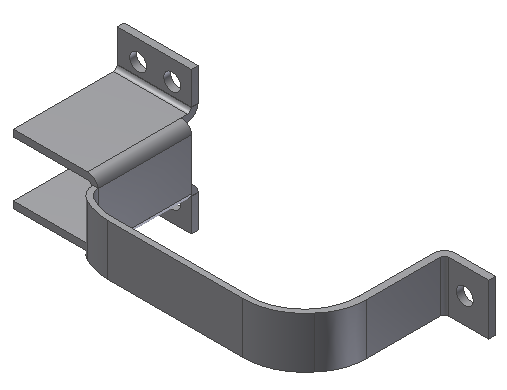
\includegraphics[width=\linewidth]{../Common/images/nonCellularBracket}}  &  
%\adjustbox{valign=t}{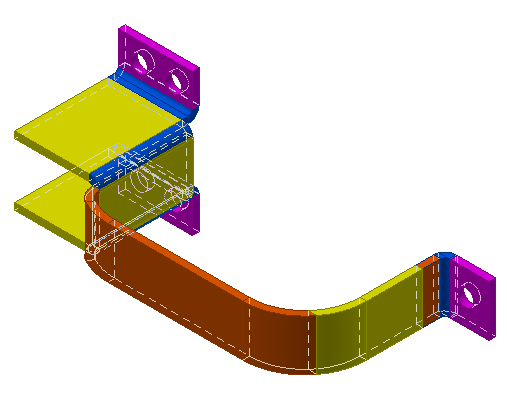
\includegraphics[width=\linewidth]{../Common/images/CellularBracket}}  &
%\adjustbox{valign=t}{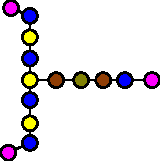
\includegraphics[width=\linewidth]{../Common/images/CellGraphBracket.pdf}} &  
%\adjustbox{valign=t}{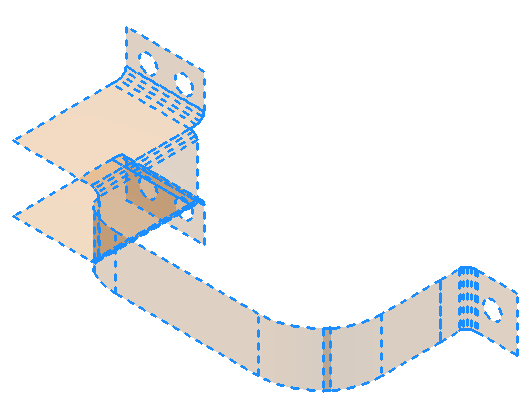
\includegraphics[width=\linewidth]{../Common/images/midsCellularBracket}} 
%\\ %\midrule
\bottomrule
\end{tabular}
}
\captionof{table}{Feature based Cellular Midsurface of Alphabets}\label{tbl_fbcmalpha}
\end{center}


\todo[backgroundcolor= yellow]{\textbf{Reviewer}:  At the end of section 2, the authors state that no heuristic rules are used. Indeed, the criteria set by the
authors about the cellular decomposition and the connection between mid­surfaces put strong restrictions on
the range of solids that can be processed. The examples used are essentially 2D type examples where
thickness is constant. \\ \textbf{Author}: Added variable thickness example}

%\subsection{Example Sheet Metal Part}
Figure \ref{fig_orig} shows a real-life part, where as Figure \ref{fig_mids} shows the output, a well-connected midsurface.

	\def\mymidsdormcolumnwidth{0.43}
\begin{figure}[!h]
\centering     %%% not \center
\subfloat[Original Part]{\label{fig_orig}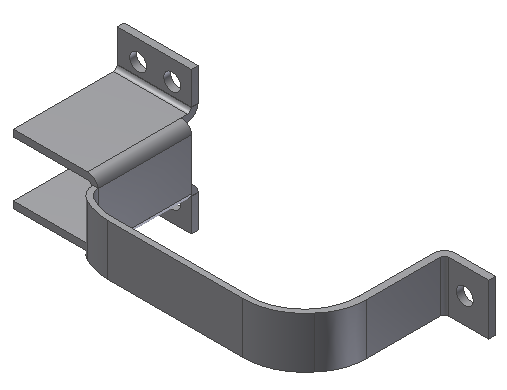
\includegraphics[width=\mymidsdormcolumnwidth\linewidth,valign=t]{../Common/images/nonCellularBracket}} \qquad
%\subfloat[Original Part]{\label{fig_orig}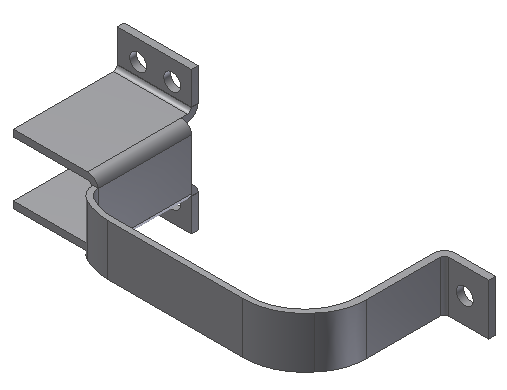
\includegraphics[width=0.25\linewidth,valign=t]{../Common/images/nonCellularBracket}}
%\subfloat[Decomposition]{\label{fig_cd}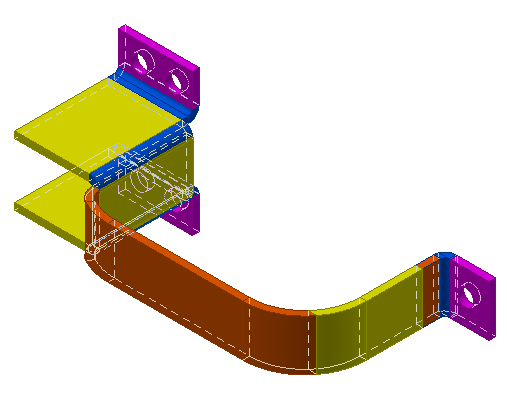
\includegraphics[width=0.25\linewidth,valign=t]{../Common/images/CellularBracket}}
%\subfloat[Exploded View]{\label{fig_expl}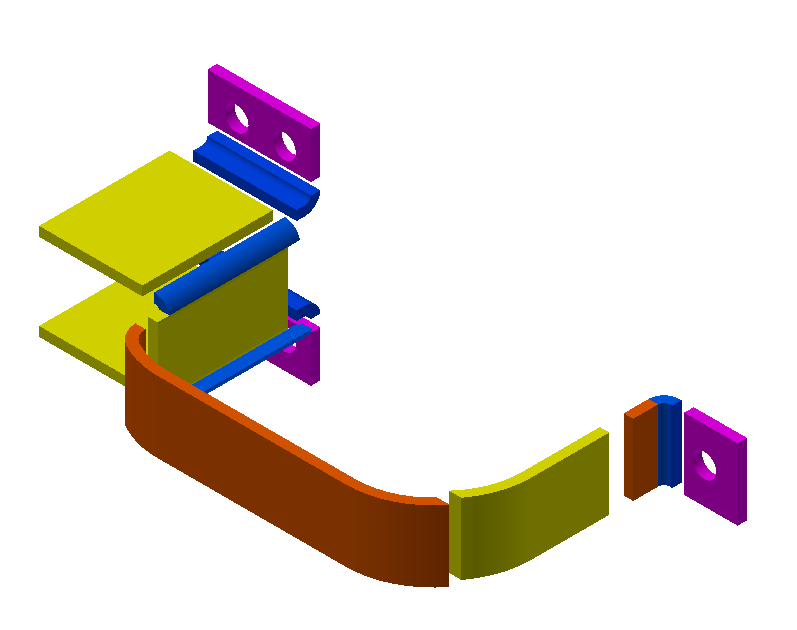
\includegraphics[width=0.25\linewidth,valign=t]{../Common/images/CellularBracketExploded}}
%\subfloat[Graph]{\label{fig_cg}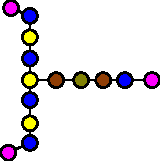
\includegraphics[width=0.195\linewidth,valign=t]{../Common/images/CellGraphBracket.pdf}}\\
\subfloat[Midsurface]{\label{fig_mids}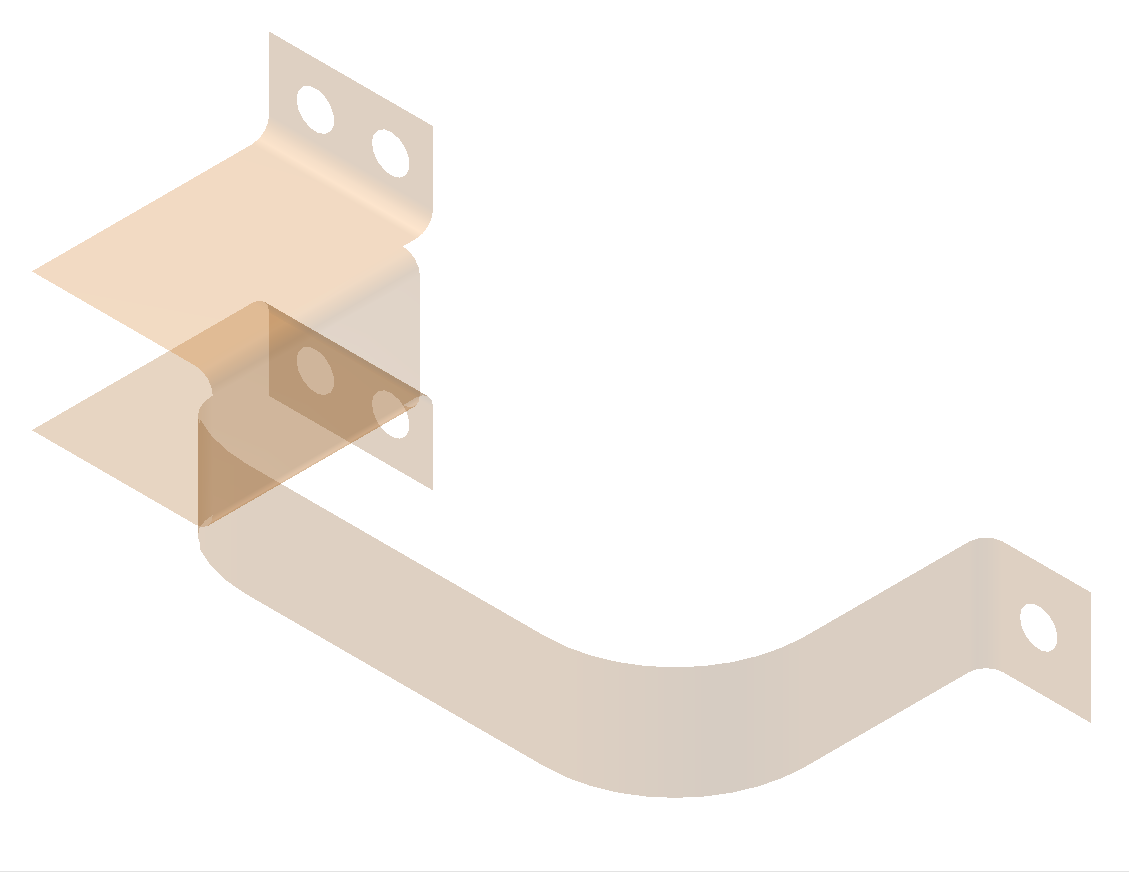
\includegraphics[width=\mymidsdormcolumnwidth\linewidth,valign=t]{../Common/images/MidsurfAfterDormant}}
\caption{Computation of Midsurface of a Bracket}
\end{figure}

\vspace{-5mm}

%\section{Validation}
%\label{Validation}
%
%Midsurface is expected to truly represent the original solid, both in terms of geometry and topology. It is tedious to follow the manual process of inspection to validate it, especially for the complex models. The present system performs such validation in an automated way and uses Hausdorff's distance measure to verify geometric correctness. However, as a necessary and sufficient validation, the system also carries out topological validation to verify the connectivity as well as missing surfaces or gaps. The following section demonstrates the formulation developed to carry out such validation (\cite{YogeshCADandA2015}). 
%
%The main idea behind the formulation is that, the generated midsurface is expected to be such that it is obtained as if the solid body is shrunk to its overall neutral plane. As a reverse validation, if such a midsurface is thickened it should represent a solid body as close as original solid as possible. Th solid's topological validity is then checked using Euler-Poincar\'e's manifold equation. If the original midsurface had any gaps or overlaps, the resultant solid will not satisfy the manifold condition. 
%
%\begin{minipage}[htb]{\linewidth}
%\centering 
%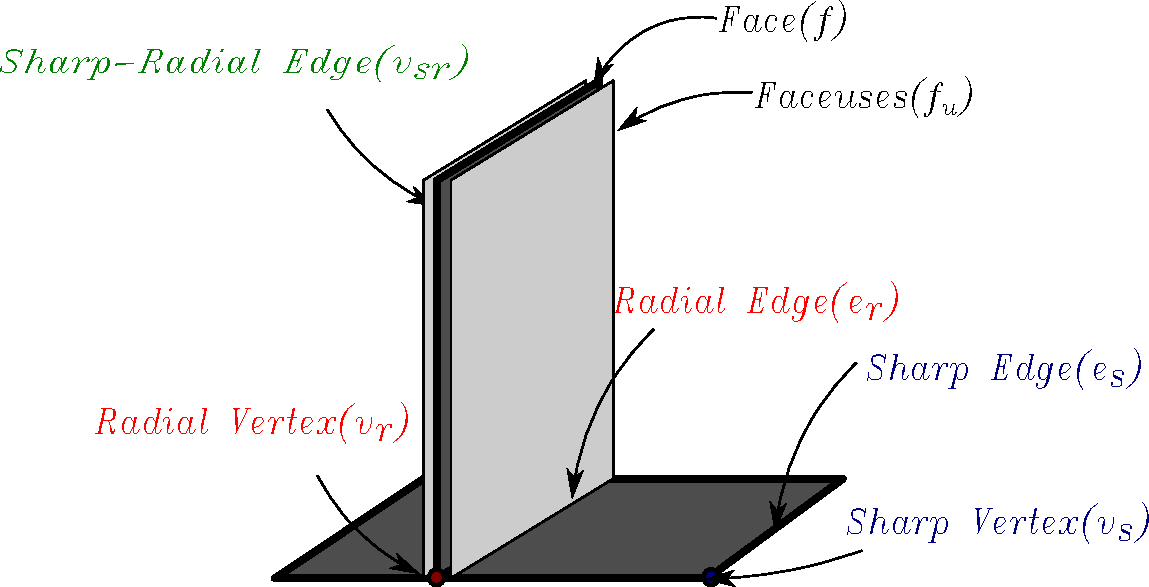
\includegraphics[width=0.7\linewidth]{../Common/images/NonManifoldT1.pdf}
%\vspace{2mm}
%\captionof{figure}{Non-Manifold topological entities}
%\label{fig_nonmanifold}
%\end{minipage}
%
%Procedure to validate midsurface is as follows (\cite{YogeshCADandA2015}):   %%%%%%%%%%% ADD in (\cite{YogeshCADandA2015}) LATER
%
%Steps:
%\begin{enumerate}[noitemsep,topsep=2pt,parsep=2pt,partopsep=2pt]
%\item Classify Midsurface entities  as : $f, e_s , e_{sr} , e_{rr}, e_r , e_i, v_s , v_r , v_i, s , h , r$ (Figure \ref{fig_nonmanifold})
%\item Predict topological entities using the equations developed  (\cite{YogeshCADandA2015})%%%%%%%%% ADD  in (\cite{YogeshCADandA2015}) LATER
%%\item Verify that the topological entities of the Midsurface satisfy the non-manifold equation, by showing that left ($\chi_{nml}$) and right  ($\chi_{nmr}$) hand side of the equation matches.
%\item Verify that the predicted topological entities of the  thin-wall solid satisfy the manifold equation, by showing that left ($\chi_{ml}$) and right  ($\chi_{mr}$) hand side of the equation matches. %Thus proving that the transformation equations are valid. 
%\end{enumerate}
%
%
%\begin{tabular}[htp]{@{}p{0.48\linewidth}  p{0.48\linewidth}@{}} \toprule
%{\bf Midsurface} & {\bf Edge Classification} \\ \midrule
%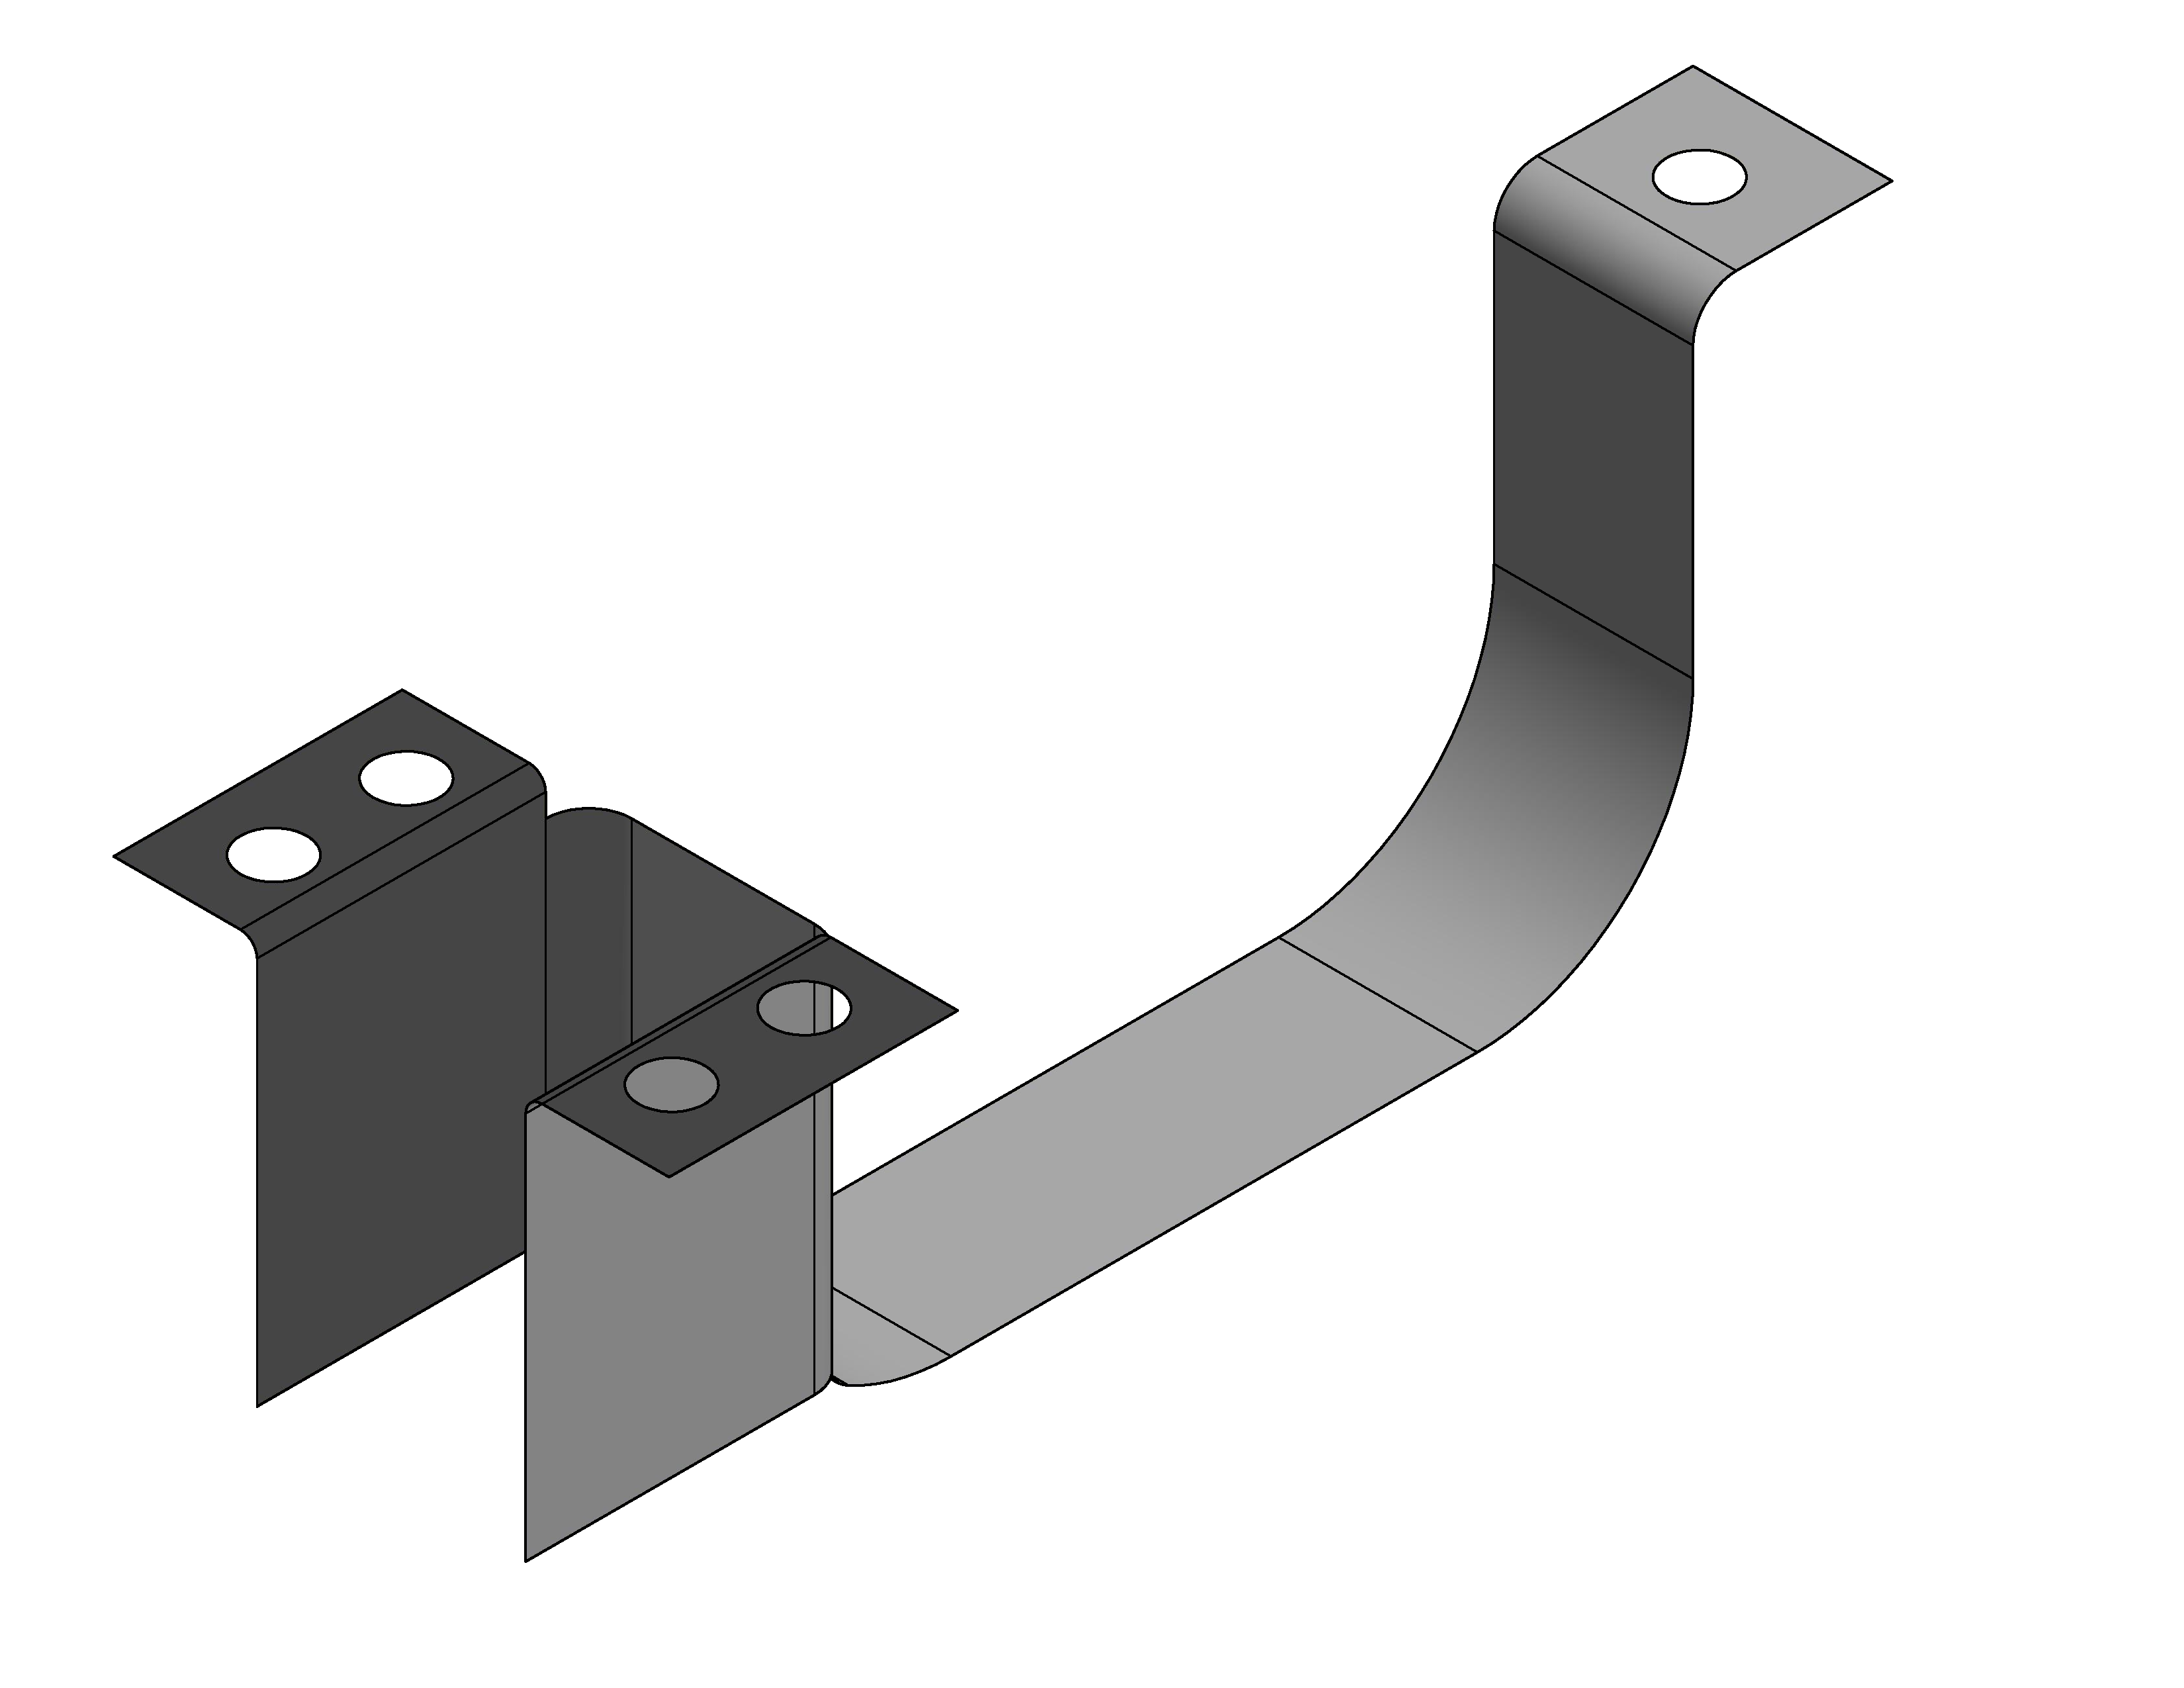
\includegraphics[width=0.8\linewidth]{../Common/images/SimpleBracketMidsurfshaded.pdf} &
%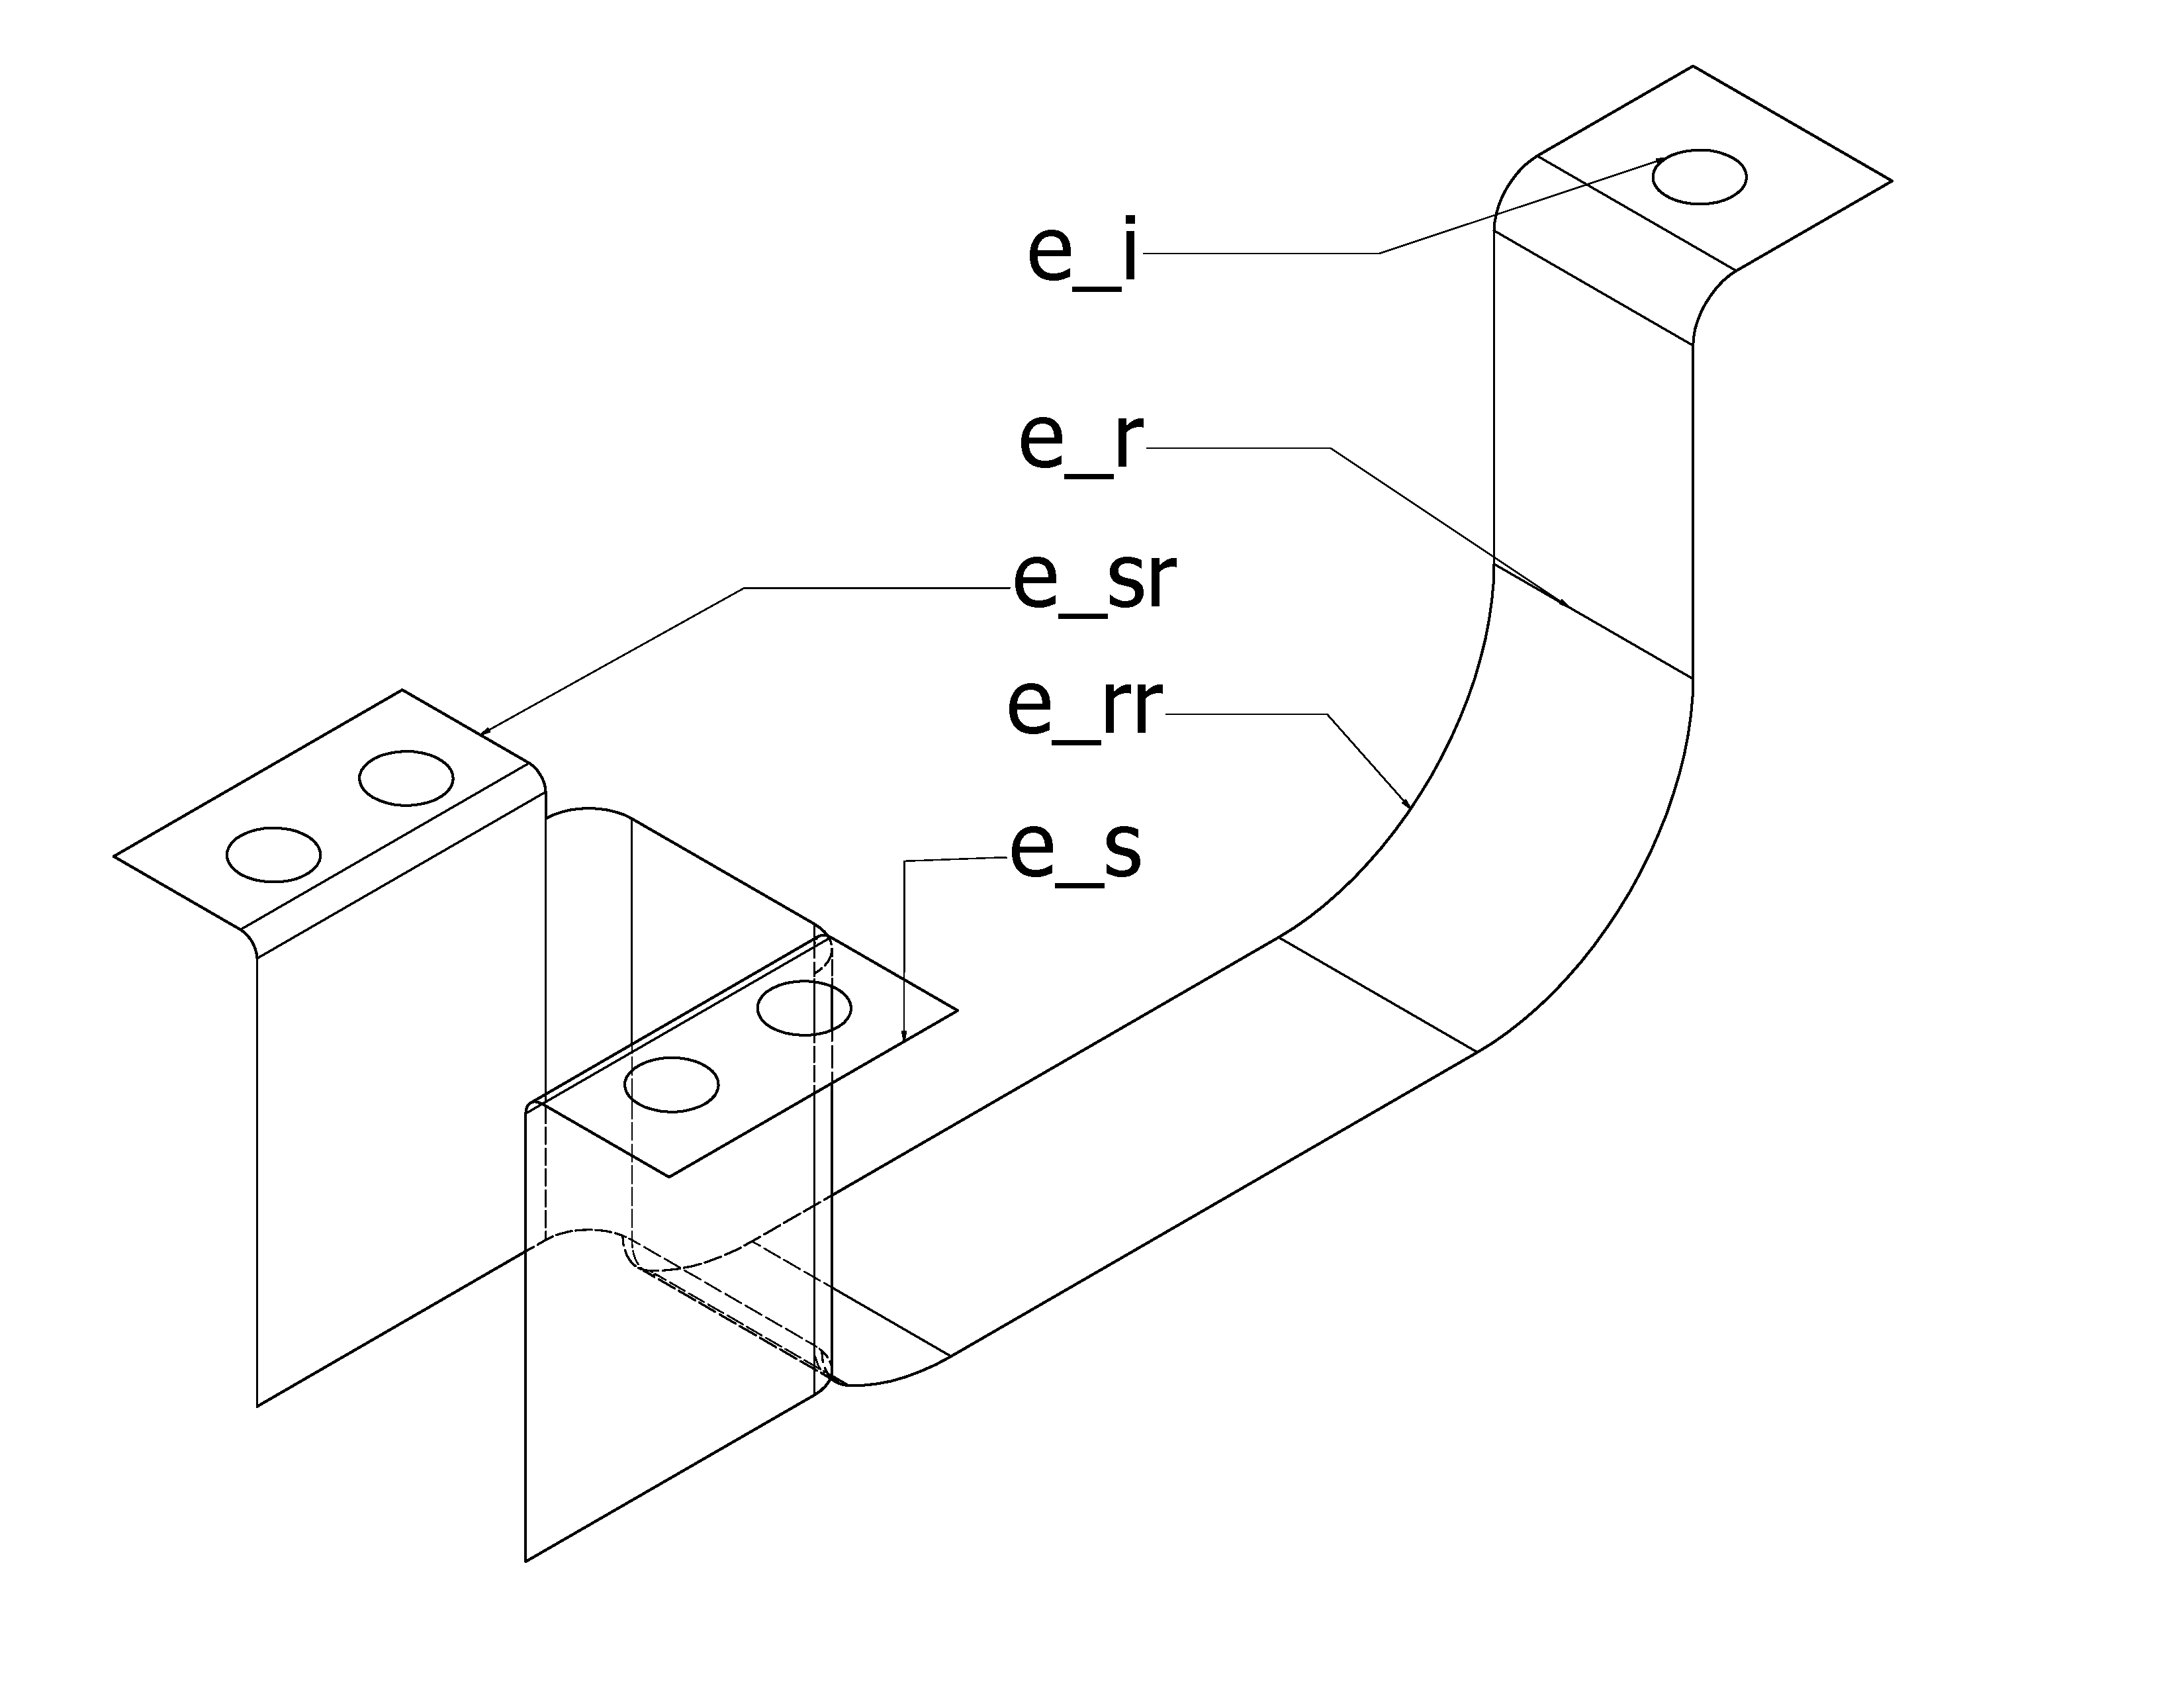
\includegraphics[width=0.8\linewidth]{../Common/images/SimpleBracketMidsurf.pdf}\\ \bottomrule
%\end{tabular}
%
%\begin{enumerate}
%[noitemsep,topsep=2pt,parsep=2pt,partopsep=2pt]
%\item \textbf{Midsurface entities}: \\$f = 15, e_s = 3, e_{sr} = 10, e_r = 14, e_{rr} = 19, l_p = 9 ,e_i=5,v_s = 8,v_r =24, v_i= 5, s=1,h=5,r=5$
%\item \textbf{Predicted solid-faces}: \\$f_m = 2f+e_s+ l_p +e_i $\\$= 2 \times 15 + 3 + 9 + 5 = 47$
%\item \textbf{Predicted solid-edges}: \\ $e_m = 2(e_s+e_{sr}+e_{rr}+e_i )+ \sum n_{r} e_{r}+v_s+v_i $\\$= 2(3+10+19 + 5)+ (2\times 12 + 4 \times 2)+8+5 = 119$
%\item \textbf{Predicted solid-vertices}: \\$v_m = 2(v_s+ v_i) + \sum n_{r} v_r$\\$=2\times (8 + 5)  + 2 \times 24=74$
%\item \textbf{Predicted solid-shells-holes}: \\$s_m =s = 1, h_m = r_i  = 5, r_m = 2r_i = 10$
%%\item \textbf{Non-manifold equation of the left side}:  $\chi_{nml} $\\$= v-e+f $\\$= 32-46+15 = 1$
%%\item \textbf{Non-manifold equation of the  right side}:  $\chi_{nmr}$\\$=s-h+r$\\$=1-5+5 = 1$
%\item \textbf{Manifold equation of the  left side}:  $\chi_{ml} $\\$= v_m-e_m+f_m $\\$=74-119+47= 2$
%\item \textbf{Manifold equation of the  right side}:  $\chi_{mr}$\\$=2(s_m-h_m )+r_m$\\$= 2(1-5)+10 = 2$
%%\item Sheet metal midsurface characteristic $\chi_{smm}$\\$=
%%e_s+e_i+(2-n_{r} ) e_{r}+e_{sr}/n_{r} $\\$=v_s+(2-n_{r} ) v_{r}+v_i$\\$ 4+0+0+0=4+0+0= 4$
%%\item \textbf{Result}: \textcolor{green}{Matches}
%\end{enumerate}
%It can be observed that the predicted solid entities validate the manifold equation ($\chi_{ml} = \chi_{mr} = 2$) and the topological entities of the thin-walled solid match with the predicted ones.
%
%Midsurface computation depends on the appropriateness of feature-generalizations as well as feature-based cellular decomposition. Sometimes, it may not be possible to abstract a form-feature in the ``Loft or Sweep'' manner, with resulting profile and guide curve.  Such complexities can be resolved by taking a hybrid approach by resorting to face-pair algorithm only at the  intricate portions.
